\documentclass[compress,handout]{beamer} %[compress,handout]

\usepackage[utf8]{inputenc}

% Mapping symbol to character in font
\usepackage[T1]{fontenc}

\usepackage[ngerman]{babel}
\usepackage[longend,algoruled,vlined,german]{algorithm2e}%[titlenumbered]
\usepackage{subfigure}
\usepackage{dsfont}
%\usepackage{hhline}
%\usepackage{colortbl}
% \usepackage{ifpdf}     % for pdflatex & pstex figures
% \usepackage{pstricks}  % wird hier nur fr die Farben verwendet
% \usepackage[svgnames]{xcolor}

% \ifpdf %
%  \newcommand{\inputfig}[1]{\input{#1.pspdftex}}%
%  \DeclareGraphicsRule{.pspdftex}{pdf}{.pspdftex}{}%
% \else%
%  \newcommand{\inputfig}[1]{\input{#1.pstex_t}}%
% \fi%

%\DeclareGraphicsRule{.pspdftex}{pdf}{.pspdftex}{}%
\newcommand{\inputfig}[1]{\input{#1.pspdftex}}%

\renewcommand{\O}{\mathcal{O}}
\newcommand{\Otilde}{\mathcal{\tilde{O}}}
\newcommand{\NP}{\ensuremath{\mathcal{NP}}}
\renewcommand{\P}{\mathcal{P}}
\newcommand{\ZPP}{\mathcal{ZPP}}

\makeatletter
% \ifcase\@ptsize
%   \font\mtimes=cmsy10 scaled \magstep3 % was 4
% \or
%   \font\mtimes=cmsy10 scaled 1577      %\magsetp3.5
% \or
  \font\mtimes=cmsy10 scaled \magstep4
%\fi
\def\bigtimes{\mathop{\lower.15\baselineskip\hbox{\mtimes\char"02}}}
\makeatother

\newcommand{\N}{\mathds{N}}
\newcommand{\Q}{\mathds{Q}}
\newcommand{\R}{\mathds{R}}

%\newcommand{\Pr}{\mathrm{Pr}}
\newcommand{\E}{\mathds{E}}

%\newcommand{\probname}[1]{\textsc{#1}}
\newcommand{\probname}[1]{\textbf{#1}}

% Volkers defs
\newtheorem{observation}[theorem]{Beobachtung}

\newcommand{\IA}[1]{\smallskip\noindent{\bf Induktionsanfang (\boldmath$#1$\unboldmath):}}
\newcommand{\IS}[1]{\smallskip\noindent{\bf Induktionsschritt (\boldmath$#1$\unboldmath):}}

% \makeatletter
% \def\case{\@ifnextchar[{\c@@se}{\c@se}}
% \def\c@se#1{\@case{Fall~#1:}}
% \def\c@@se[#1]#2{\@case{Fall~#2 (#1):}}
% \def\@case#1{\par\smallskip\noindent\boldmath{\bf#1\ }\unboldmath\ignorespaces}
% \makeatother

%\def\argmax{\mathop{\operator@font argmax}}
\def\argmax{\mathop{argmax}}
%\def\argmin{\mathop{\operator@font argmin}}
\def\argmin{\mathop{argmin}}
\def\floor#1{\lfloor#1\rfloor}
\def\ceil#1{\lceil#1\rceil}
\def\Floor#1{\left\lfloor#1\right\rfloor}
\def\Ceil#1{\left\lceil#1\right\rceil}
\def\ament#1#2{\left(#1\atop#2\right)}
\def\cdotfill{\leaders\hbox to .4em{\hfil$\cdot$\hfil}\hfill}
\def\dashfill{\leaders\hbox to 1em{\hfil$-$\hfil}\hfill}

%\def\opt{\mathop{\operator@font opt}}
\def\opt{\mathop{opt}}

\newcommand{\rvec}[3]{(#1_{#2}, \ldots ,#1_{#3})}
\newcommand{\word}[3]{#1_{#2} \cdots #1_{#3}}
\newcommand{\setsep}{\mathchoice{\::\:}{\,:\,}{:}{{:}}}
\newcommand{\set}[2]{\left\{#1\setsep#2\right\}}
\newcommand{\pp}{\raisebox{1.5pt}{$\scriptstyle++$}}
\newcommand{\mm}{\raisebox{1.5pt}{$\scriptstyle--$}}

\newcommand{\problemdesc}[4]{
\begingroup\clubpenalty10000\widowpenalty10000
%\par\vskip\topsep\vskip\partopsep\par\noindent
\begin{problem}
\noindent\underline{\scshape#1\strut\label{#2}}%
\par\nobreak\vskip.2\baselineskip
\setbox0\hbox{\bf Eingabe: }\dimen0=\wd0
\setbox1\hbox{\bf Gesucht: }\ifnum\wd1>\wd0\dimen0=\wd1\fi
\advance\dimen0 by 2pt
\vskip-\parskip\noindent
\hbox to\dimen0{\box0\hfil}\hangindent\dimen0\hangafter1\ignorespaces#3
\par\vskip-\parskip\noindent
\hbox to\dimen0{\box1\hfil}\hangindent\dimen0\hangafter1\ignorespaces#4
\end{problem}%
%\par\vskip\topsep\vskip\partopsep\par
\endgroup}

% \newrgbcolor{red}{1.0 0 0}
% \newrgbcolor{mediumgray}{0.5 0.5 0.5}
% \newrgbcolor{darkgreen}{0.0 0.6 0.0}


\mode<presentation>
{
  \usetheme[]{Warsaw}
%   \usetheme[]{Boadilla}
%  \usetheme[]{Copenhagen}
%  \useoutertheme{infolines} % show only current (compressed) section/subsection
  \setbeamercovered{transparent}
}

% \input{tumlogo}

\title[Enhanced and Extended Suffix Arrays]{Enhanced and Extended Suffix Arrays}
%\subtitle{String Matching}

\author[A. Regenfuß]{Adrian Regenfuß}

\institute[TUM]{
  Technische Universität München
}

\date[SS'20]{Sommersemester 2020}

\subject{String Matching}
\keywords{string matching, bioinformatics, algorithms}

% \titlegraphic{\oTUM{1cm}}

% \logo{\TUM{0,5cm}} % does not work (?), see author

\beamerdefaultoverlayspecification{<+->}

% \includeonlylecture{lec-2016-10-18}

\AtBeginSection[]% nichts tun bei *-Form (\section*{})
{
	\begin{frame}
		\frametitle{Übersicht}
		\tableofcontents[currentsection,hideothersubsections]
	\end{frame}
}

\begin{document}

\frame{\titlepage}

%% Proseminar 1 - 18.10.2016
\lecture[11.07.2020]{Vorlesung vom 11.07.2020}{lec-2020-07-11}

\section{A Personal Anecdote}

\begin{frame}
	\frametitle{4 years ago}
	\begin{itemize}
	\item Me in Nepal
	\item No computer with me, only pen, paper and Programming Pearls
	\end{itemize}
\end{frame}

\begin{frame}
	\frametitle{My old, damaged copy of Programming Pearls}
        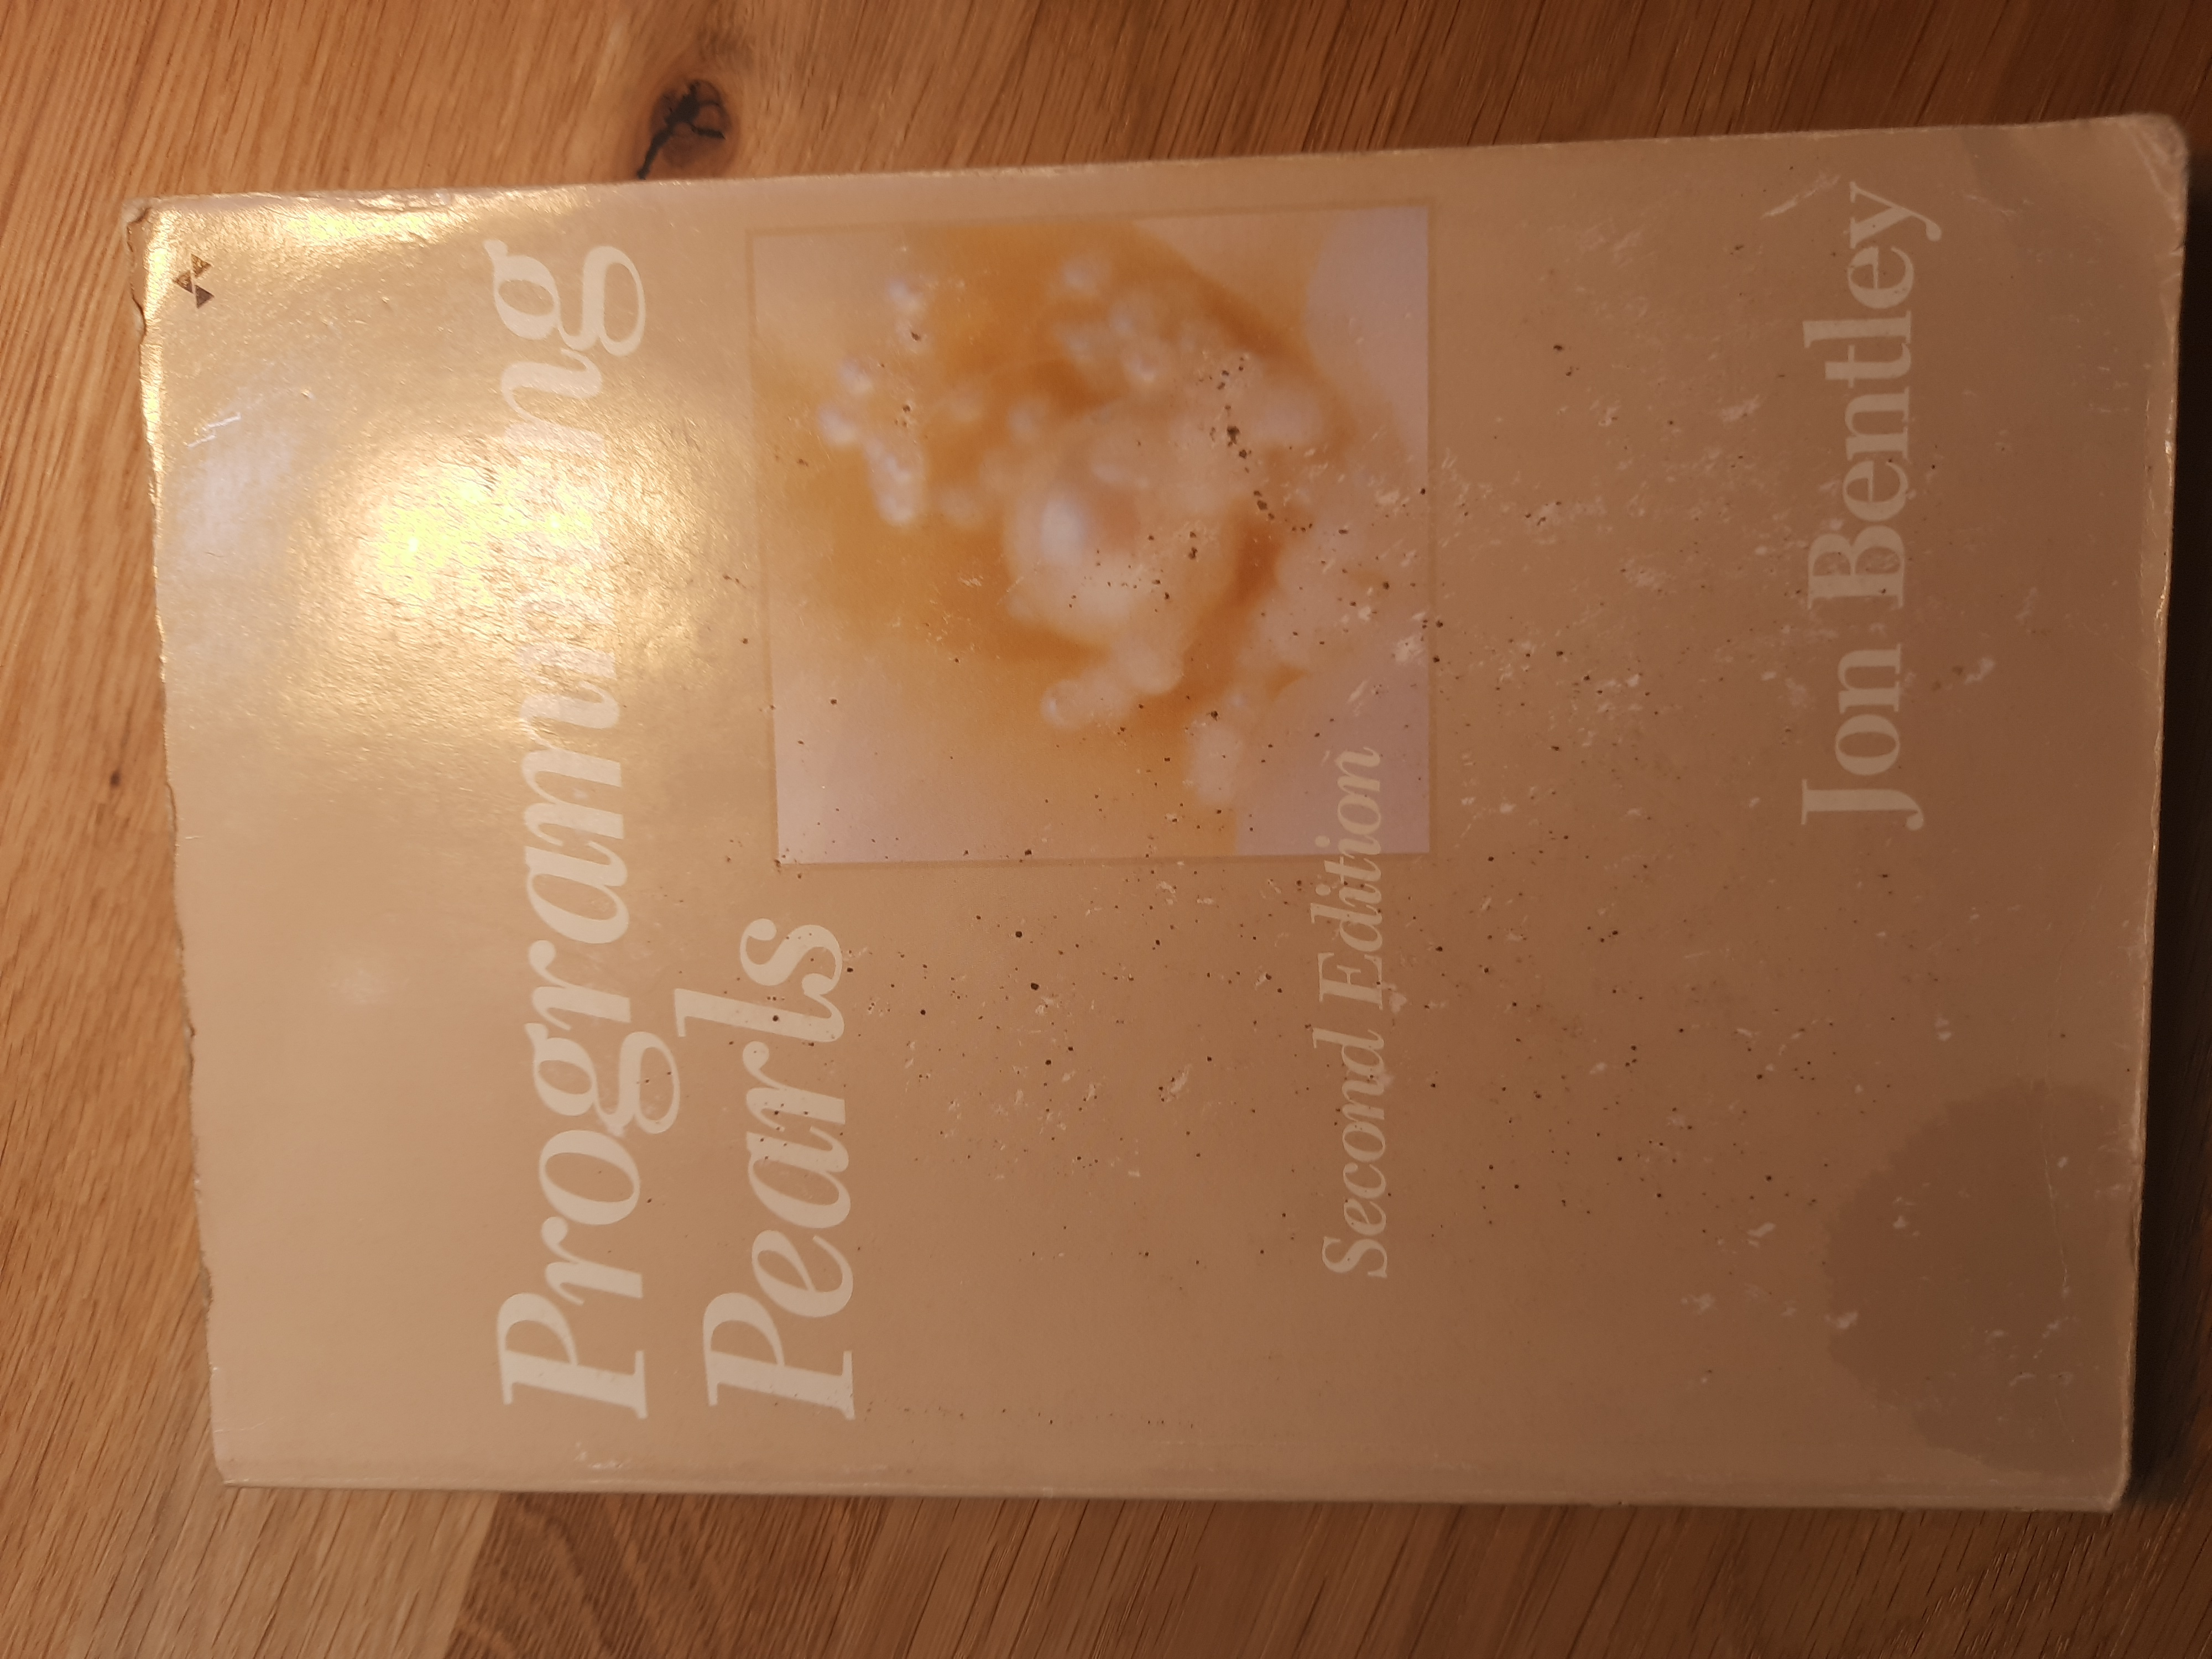
\includegraphics[width=\textwidth, height=\textheight, keepaspectratio=true]{programming_pearls}
\end{frame}

\begin{frame}
	\frametitle{Thinking a lot about Algorithms}
	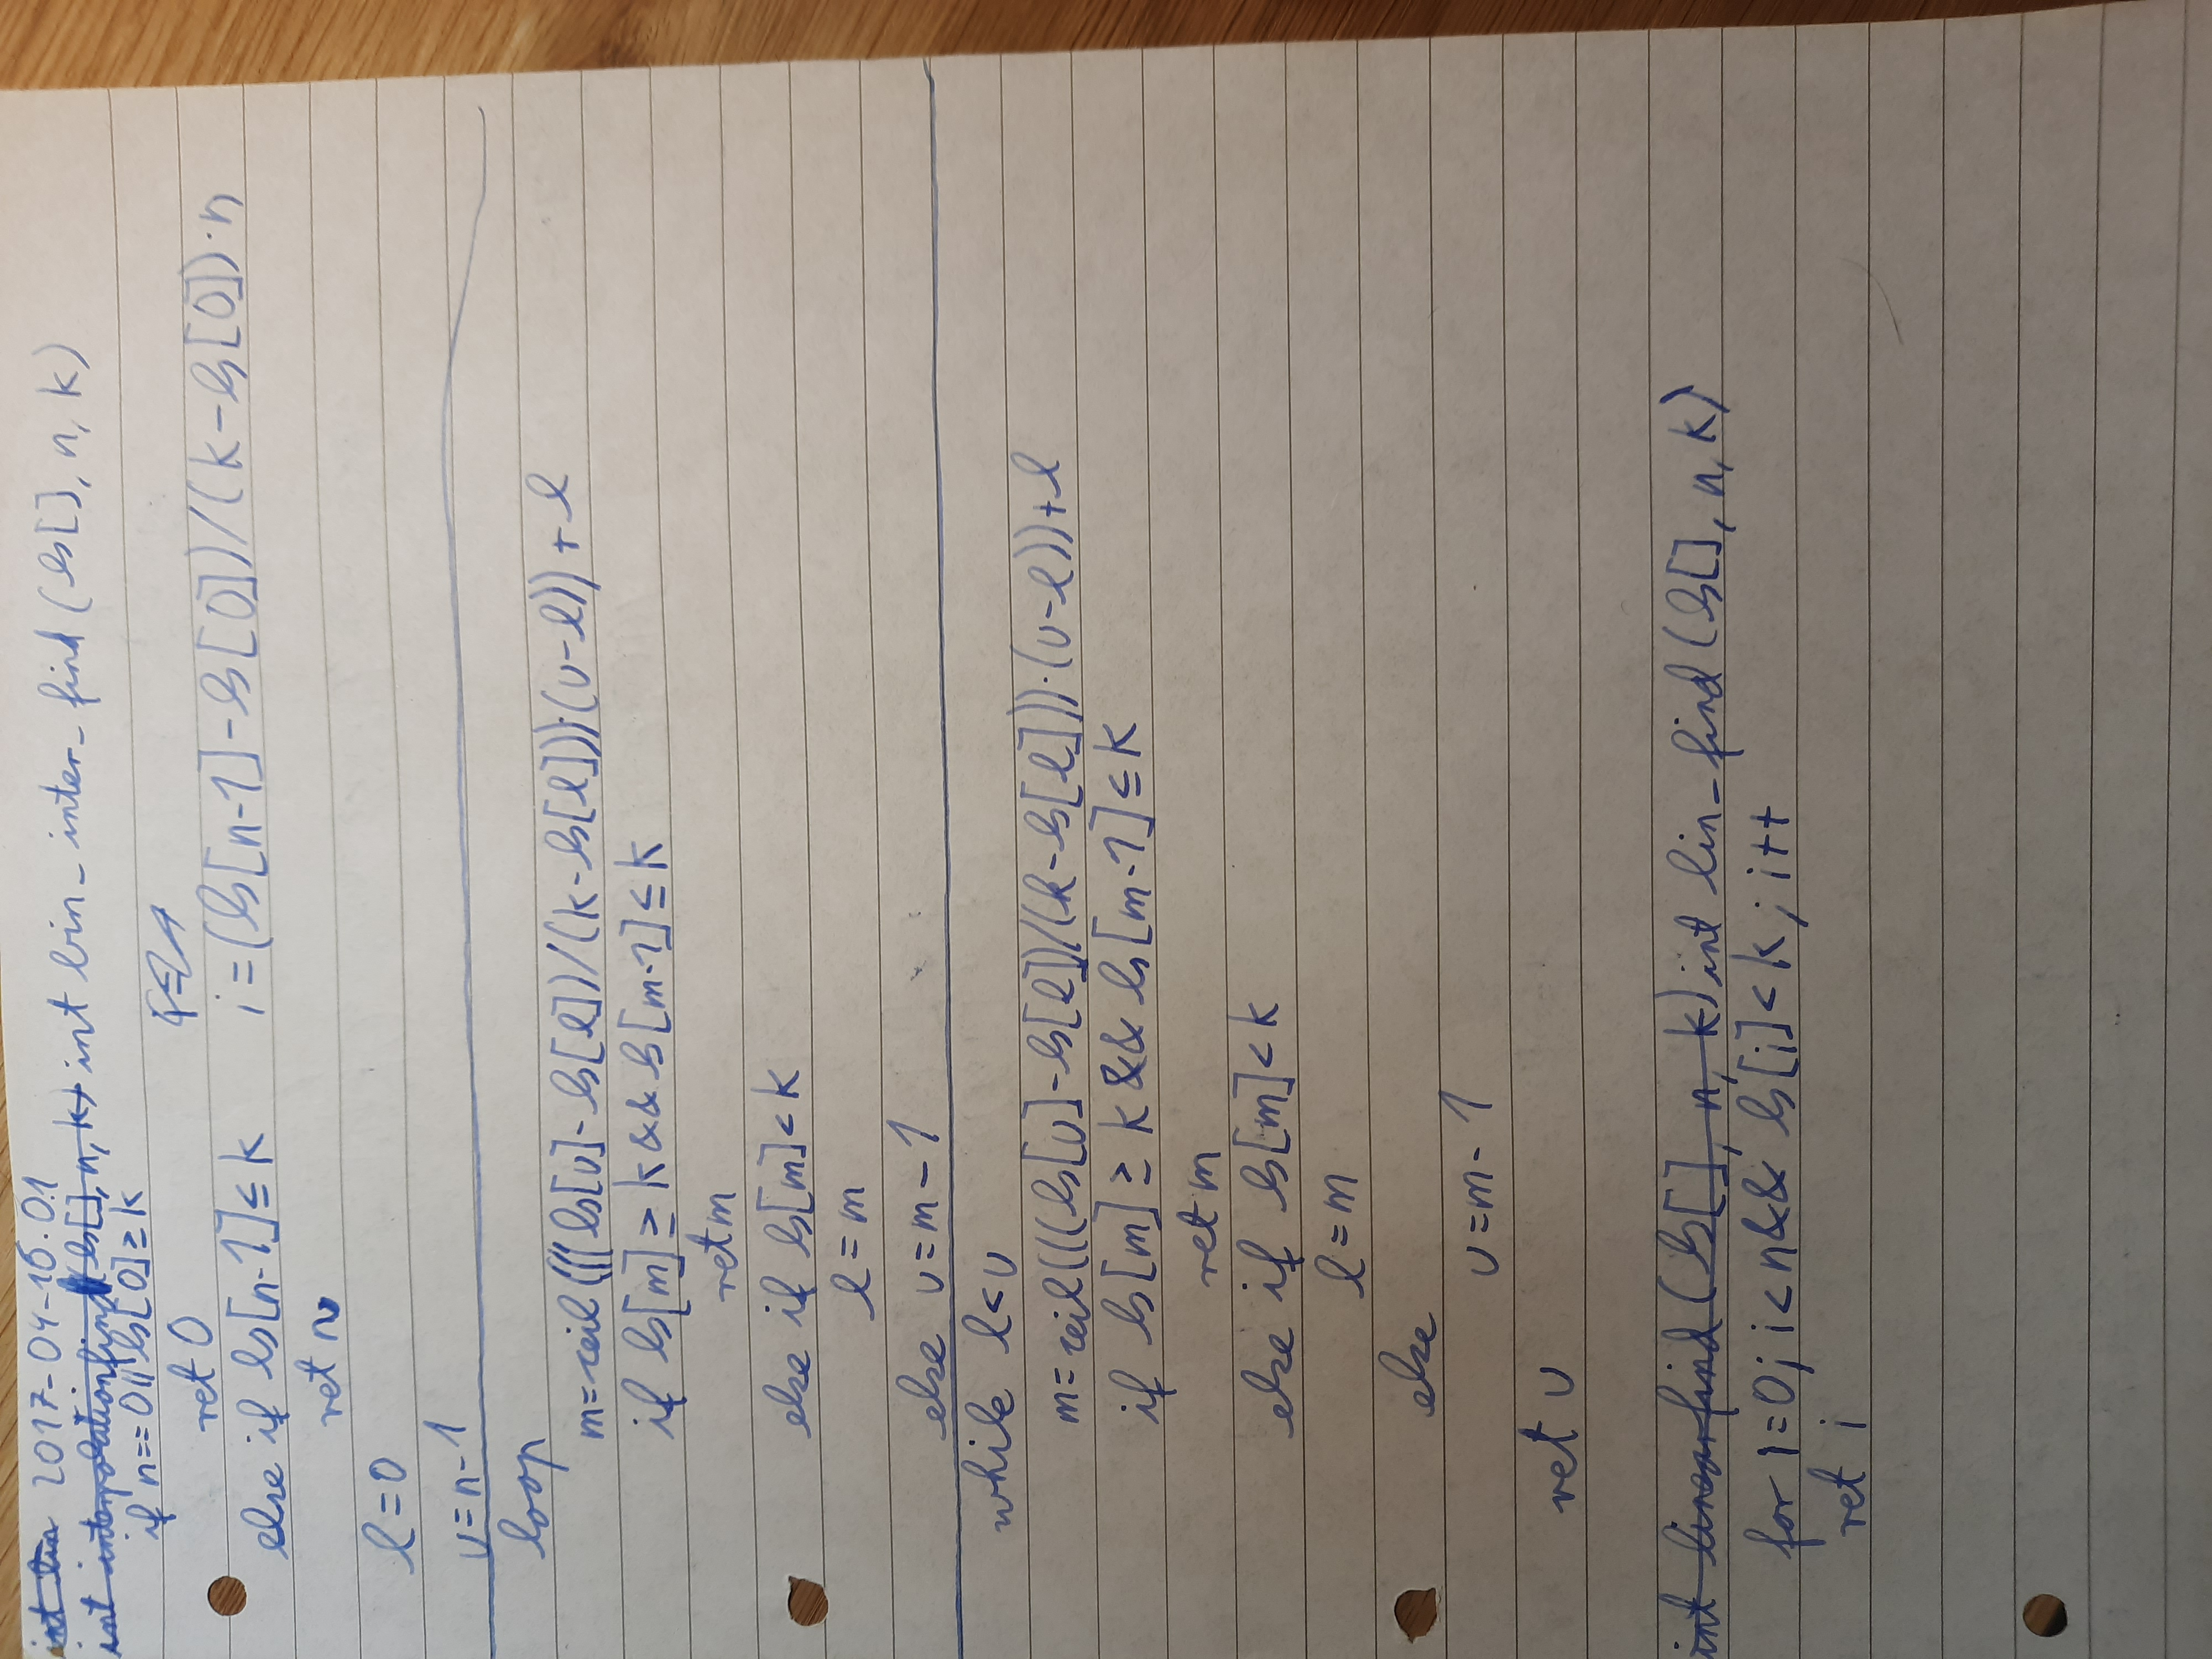
\includegraphics[width=\textwidth, height=\textheight, keepaspectratio=true]{nepal_search}
\end{frame}

\begin{frame}
	\frametitle{Problems back then}
	\begin{itemize}
		\item Thinking about searching, sorting, collision detection, string matching
		\item Specifically: What is the longest repeated substring of a string?
		\item Or: what is the longest supermaximal repeat of a string?
		\item Devising very complex algorithms
	\end{itemize}
\end{frame}

\begin{frame}
	\frametitle{Discovering Suffix Arrays}
	\begin{itemize}
		\item On the flight back reading the 15th chapter of Programming Pearls
		\item Describes this exact problem, solved using suffix arrays
	\end{itemize}
\end{frame}

\section{Structure}

\begin{frame}
	\frametitle{Structure}
	\begin{itemize}
		\item Description of data structures
		\item Clarification of terminology
		\item Description of algorithms
		\item Discussion of advantages/disadvantages
	\end{itemize}
\end{frame}

\section{Data Structures}

\begin{frame}
	\frametitle{Suffix Array}
\end{frame}

\end{document}

\section{Algorithms}

\section{Comparison with the Suffix Tree}
%%% Local Variables: 
%%% mode: latex
%%% TeX-master: t
%%% End: